\chapter{The Database}
\label{chap:database} 
In this chapter the database design and implementation hereof are explained. We will presents the ER-schema with our design and explain some of the design decision. Then we will shown the database scheme created from the implementation and explain some of the implementation decisions there have been made. Code samples will be shown from the function that update the simpler objects and finally there will be code from updating a rule.  
  
\section{Design}
\label{sec:DBdesign}
In the parent control system there are seven essential objects; control system, profile, tag, controller, chore, rule and permission. 

\begin{description}
	\item[Control system] is identifying the individual system and all of the other objects are connected to a control system.
	\item[Profile] is a representation of a specific person in the control system. The person can either be a child or the parent, but this should be distinguishable.
	\item[Tag] identifies the physical tag that a profile uses to activate the controllers. A tag is identified by the serial number of the physical tag.
	\item[Controller]	is an object representation of the physical controller and like the tag it is identified by the serial number of the physical controller.
	\item[Chore] is a representation of a house chore which can be carried out by a child (profile) which then gets points as a reward.
	\item[Permission] is representing restrictions on a controller which some of the profiles need to abide by. 
	\item[Rule] is representing other restrictions or rules that cannot be expressed by the permission. A rule consist of some conditions that need to be meet before some actions should be taken as explained previously in section \vref{sec:rule}. 
\end{description}

From the former description the database design is made. It is represented in an ER-diagram in figure \ref{fig:ERdiagram} where the cardinality ratio is expressed in Chen notation\citep{DatabaseKilde}. It should be mentioned that the design of a rule in the database is based on the first design of the rules, which can be found in appendix \vref{appendixFirstRuleDesign}. The reason for not using the final design is that it was changed far into the implementation phase and the first database design does still support the final design of rule. 

\begin{figure}
	\centering
		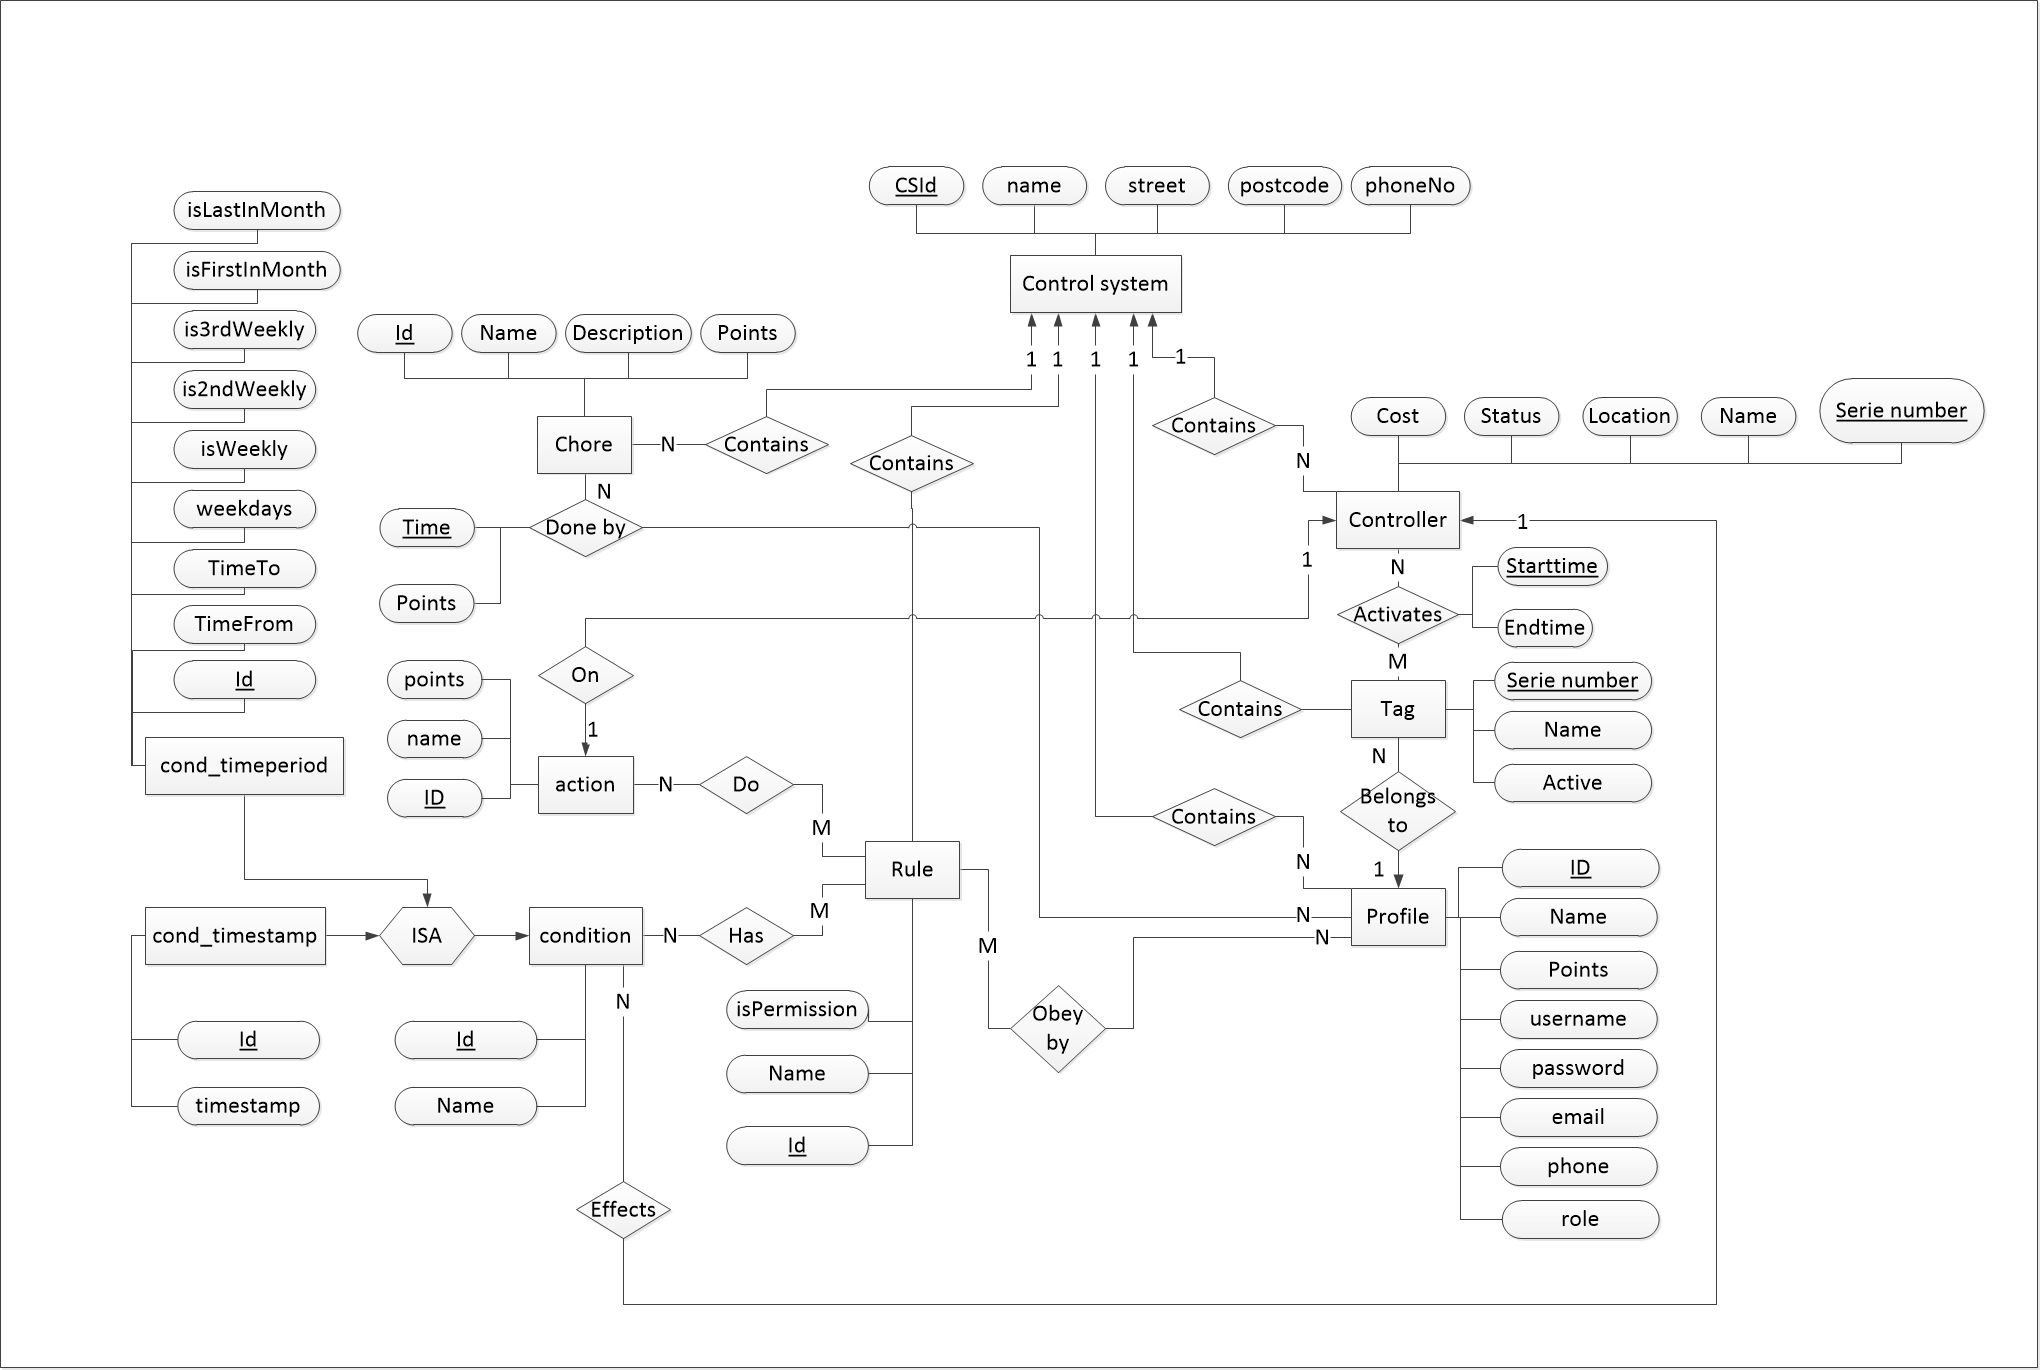
\includegraphics[width=1.50\textwidth,  angle=90]{images/ERdiagram.jpg}
	\caption{ER schema of the database design}
	\label{fig:ERdiagram}
\end{figure}

In the ER-diagram it should be noticed that Permission is absent. The reason is for every permission that could be made then there is an equivalent rule. Therefore the data representation of Permission is the same as Rule. However, on the website the two should be represented differently and so the attribute \texttt{isPermission} have been added to Rule which will differentiate the two.

Another observation from the diagram is the condition of a rule. The condition can be one of three representations. The first is the simplest because it is just the Condition. The second is Condition and a timestamp which is the \texttt{cond\_timestamp} in the design in figure \ref{fig:ERdiagram}. The last representation is Condition, a time period, and a representation of when it is valid, which in the ER-diagram is \texttt{cond\_timeperiod}. The type of condition that should be used, can be distinguished by the condition name. If the name is \texttt{Timestamp} it should be cond\_timestamp, if it is \texttt{Timeperiode} then it is cond\_timeperiod and any other name it is only the Condition. 

Notice if the database design had been designed from the final design then the table \texttt{cond\_timestamp} would not have been in the design.
After the database design had been completed it was implemented into a MySQL database.  

\section{Implementation}

The database design has been implemented in a MySQL database and the result can be found in figure \ref{fig:databaseDiagram}. In the implementation of the database redundancy and anomalies is to be avoided and null values reduced. 
The mapping from the ER-diagram to the relation representation in the database is a basic mapping according to the relations $1:1$, $n:1$, $n:m$ except for Condition which is clarified in the following section. \citep{DatabaseKilde}

\begin{figure}
	\centering
		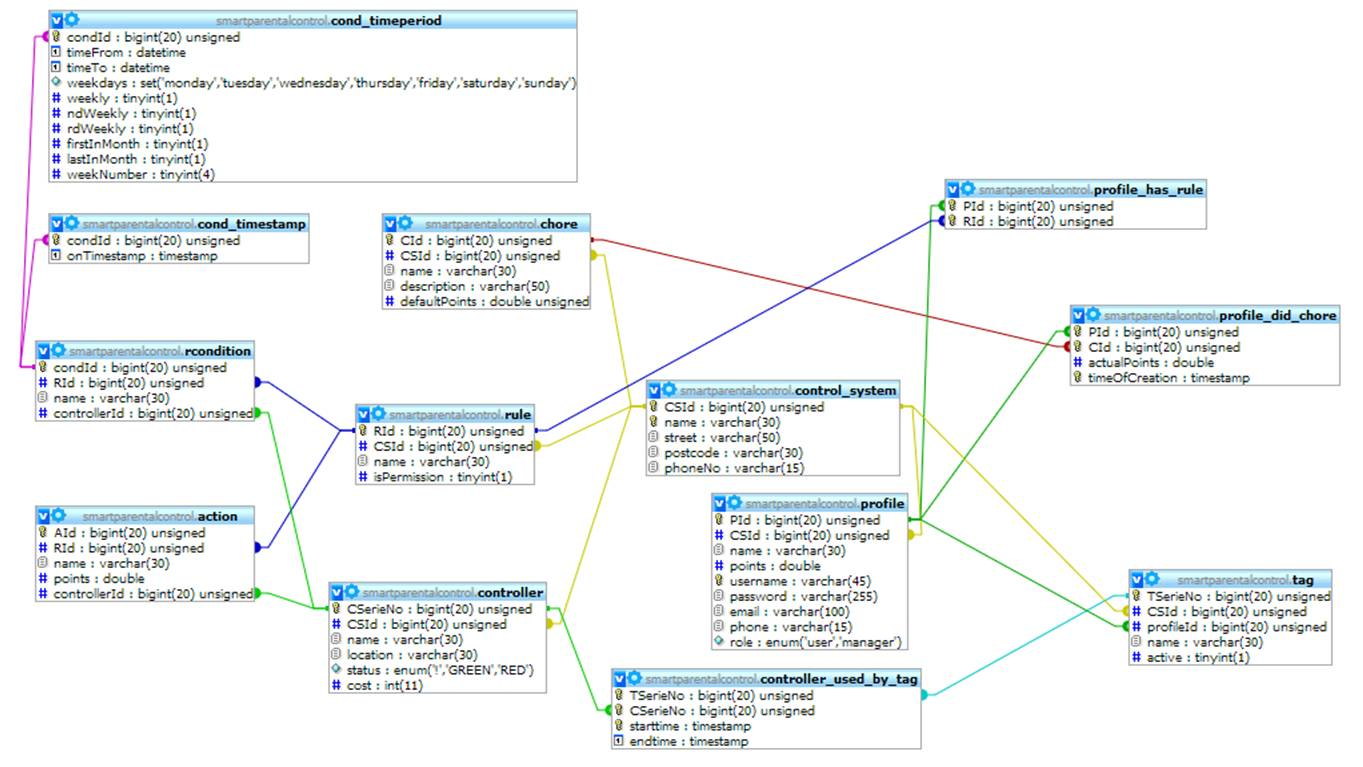
\includegraphics[width=1.50\textwidth,  angle=90]{images/databaseDiagram.jpg}
	\caption{The Database implementation}
	\label{fig:databaseDiagram}
\end{figure}

\subsection{Mapping of Condition}
\label{subsec:mappRule}
%sql or diagram
The relational modeling of Condition is more advanced because it uses generalization and as such there is a implementation choice to be made. There are four typical methods of how to deal with generalization and a solution of using each method is described below.\citep{DatabaseKilde}

\begin{description}
	\item[Using main classes,] then Condition is split up into three tables rcondition, cond\_timestamp and cond\_timeperiod where all attributes in Condition are repeated in each table. An disadvantage of using this method is in querying because it is possible to go though all three before finding the wanted data.
	\item[Using partitioning,] there are three tables rcondition, cond\_timestamp and cond\_timeperiod. The common attributes are in Condition and via an id the possible additional data can be found in either cond\_timestamp or cond\_timeperiod.
	\item[Using full redundancy,] it is much like the first, but all conditions from cond\_timestamp and cond\_timeperiod are also represented in Condition, without the additional data. As the name suggest this causes redundancy which is best to be avoided.
	\item[Using a single relation,] such that there will be a single table with all attributes from Condition, cond\_timestamp and cond\_timeperiod in the ER-diagram. It is easy to use but it will increase the number of null values. 
\end{description}

As can be see in the figure \ref{fig:databaseDiagram} the partitioning option is used in our implementation since it does not causes any redundancy or null values and it is easier to search for conditions compared to using the main classes. However, using partitioning there will be some challenges in making the functions to insert, update and get data about the rules, as will be explained in section \vref{subsec:dbRule}.\\\\

There have also been made an important decision about how to deal with deletion of data from the essential tables and this is explained in the following section.
 
\subsection{Deleting in the database}
%delete cascade
When a tuple in one of the tables control\_system, profile, tag, controller, chore, and rule should be deleted it will likely affect data from another table because of the foreign keys. We have made an intentionally decision to use \texttt{ON DELETE CASCASED} with all foreign keys, because in any case when deleting a tuple from the essential tables its history is irrelevant and should be deleted.\\
\\
As a consequence of this decision if a control system is deleted then every profile, tag, controller, chore, and rule that is connected to control system will be deleted. If a profile is deleted then this profile's tags will be deleted including all of its history, such as when the tag have been used to activate the controllers, or when the user have done a chore.
 So it is very important that when data is to be deleted then it should not be regretted later.  \\\\

However, for anything to be added, updated or deleted by the user the website need a connection to the database which is done through the class MySQLHelper. 

%sql Helper class
\subsection{MySQLHelper class}
The website and API for the controllers connect to the database by using a PHP class MySQLHelper, which establish a connection and send queries to it. The class have a construct and destruct that respectively establish the connection and close the connection to the database. The queries also go through this class in at least one of these methods:

\begin{description}
	\item[insertInto] this makes a SQL string to insert into the database.
	\item[update] this make a SQL string to update data in the database.	
	\item[delete] this make a SQL string to delete data in the database.
	\item[query] this make a SQL query string.
	\item[executeSQL] this sends the query to the database and returns the result. All of the above uses this method.
\end{description}
  
It is also possible to control the transactions through this class by disabling the auto-commit of transactions and then manually commit when it is necessary. \\\\

This class is used by several functions that are connected to the website and API. In the following section we present the more interesting of them, how to update rules. 

\subsection{EditRule from the Function Library}
\label{subsec:dbRule}
%if someday our repport gets to long this can be cut out or reduced
This system also have a function library which can get, insert, update or delete data from the database. Among these functions are e.g. \texttt{simpleInsertIntoDB} and \texttt{simpleUpdateDB} that is used to insert and update the essential tables with the exception of Rule. Insert and updating a rule is similar but the latter is the more interesting so it will be this sections focus. 

As stated previously in mapping of a rule in subsection \vref{subsec:mappRule}, there would be some challenges to make the insert and update functions. This is partly due to the fact that the data of a condition  is one of two alternative: condition, condition plus timestamp  or condition plus timeperiod as was explained in section \vref{sec:DBdesign}. However, in the newer design of a rule the condition plus timestamp is removed which makes it easier, but the problem still exists. In update it is also a challenge that each condition and action can be removed, add or updated which all should be handled together and this will be explained further in this section. 

The function to update a rule is called editRule and it also uses some other function as described below:

\begin{description}
	\item[addAction] from a rule id and an object of type Action it adds an action to the rule.
	\item[editAction] from an object of type Action it updates the attributes in the database.   
	\item[addCondition] from a rule id and an object of type Condition adds a condition to the rule.
	\item[editcondition] from an object of type Condition it updates the attributes in the database.   
\end{description}

The editRule has three inputs a Rule object, an array with Condition objects, and an array with Action objects. First the rule data will be update and then each condition and action must also be updated. 

However, when updating an action and especially a condition the changes can have different characteristics as listed below. This is also in the decision diagram in figure \ref{fig:updateRule}.

\begin{itemize}
	\item a new condition or action is added.
	\item a condition or action need to be deleted.
	\item an existing condition or action is to be updated with no structural change in the database.
	\item an existing condition or action is to be updated but with a structural change in the database.
\end{itemize}

With a structural change it is meant that the name of the condition or action has been changes and this change can influence e.g. whether cond\_timeperiod or cond\_timestamp should be used. As a result it have been decided that in this case the old condition should be deleted and the new be added anew. A structural change should not happen for an action, but the functions are still able to handle it in the same way as a condition.

\begin{figure}
	\centering
		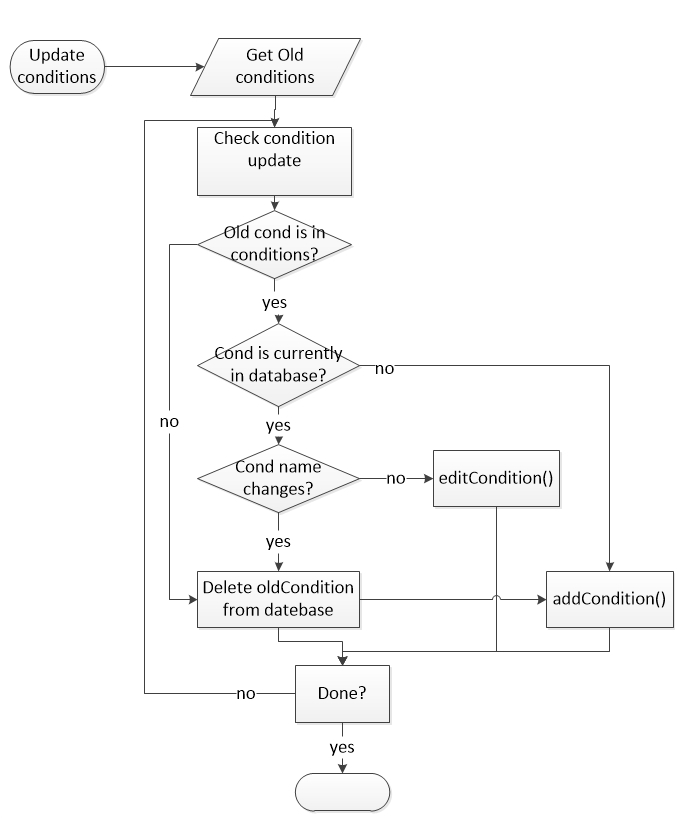
\includegraphics[width=0.75\textwidth]{images/updateRule.jpg}
	\caption{updateRule}
	\label{fig:updateRule}
\end{figure}



%
%The code sample in \ref{code:UpdateRules} is from the update handling of condition and the it is similar to handle the actions. First the old conditions id are need such that they can be compared to the ids of the Condition objects from the array \$arrayOfCondition, see line $2$. 
%Then foreach old condition id we will look thourgh the new id and if it found and the name are not to be changed then we call editcondition with the updated condition object and remove this object from the array of condition, see line $4-20$. 
%From line $22-26$ it is shown that the tuple with the old id is removed if no match was found among conditions in the array or if a match was found but the name are to changed. Now all the condition that was intended to be deleted is gone and finally the remain objects is then add or re-add from the array with addCondition, see line $28-40$.
%
%
%\begin{lstlisting}[language=PHP, label=code:UpdateRules, caption=editRule code sample]
%//SELECT condId AS id FROM rcondition WHERE RId = ($ruleData->RId)
%$CondIdResult = $db->query($theColumns['Rcondition'][0].' AS id', $theTables['Rcondition'], $theColumns['Rcondition'][1] . " = " . $ruleData->RId );
				%
	%while($row = mysqli_fetch_assoc($CondIdResult))
	%{
		%$StillExists = false;
		%foreach($arrayOfCondition as $key => $cond)
		%{
			%if($row['id'] == $cond->condId && $cond->name == null)				//edit the condition in db
			%{
				%$StillExists = true;
				%$tempresults = editCondition($cond);
				%unset($arrayOfCondition[$key]);
				%if(is_string($tempresults))
				%{
				%//if not bool then it is an error message
					%return $tempresults;
				%}
			%}	
		%}
		%//row id is not among the updated condition or cond_name not null so delete 
		%if(!$StillExists)
		%{
			%$db->delete($theTables['Rcondition'], $theColumns['Rcondition'][0] . " = " .$row['id']);
		%}
	%}
	%//add the remaining condition to db
	%if($arrayOfCondition != null )
	%{
		%foreach($arrayOfCondition as $cond)
		%{
			%//if a new condition should be added then make condition here
			%$tempresults = addCondition($ruleData->RId, $cond);
			%if(is_string($tempresults))
			%{
			%//if not bool then it is an error message
				%return $tempresults;
			%}
		%}
	%}
%\end{lstlisting}

\subsubsection{Status on Database and Function Library}

The database and the functions mentioned have all been made prior to when the decision of the rule's design changed. The functions which uses condition can now be further improved but this will not be done because it is not a priority since these functions still meet the requirements of the system.

Up till now the rules could have several conditions and actions but late in the implementation of the Website we have decided to only allow one action and condition per rule to get a more user-friendly website, more about this decision can be found in section \vref{subsec:rulesWEB}. Most functions are still implemented on the first design so they can handle several conditions and actions. 

However, a few functions can only work with one condition and action per rule. An example is the function that checks whether a user can use a media, called $db\_rules\_user\_can\_turn\_device\_on$. If the implementation of rules on the website is changed a new version of these functions need to be made.
